
%% Modern Physics Questions used on the
%% NYSED Physics Regents Examination
%%--------------------------------------------------

%% this section contains 96 problems


%% Section June2015
%%--------------------
\element{nysed}{
\begin{question}{June2015-Q50}
    What is the quark composition of a proton?
    \begin{multicols}{2}
    \begin{choices}
      \correctchoice{uud}
        \wrongchoice{udd}
        \wrongchoice{csb}
        \wrongchoice{uds}
    \end{choices}
    \end{multicols}
\end{question}
}


%% Section June2014
%%--------------------
\element{nysed}{
\begin{question}{June2014-Q15}
    Two pieces of flint rock produce a visible spark when they are struck together.
    During this process,
        mechanical energy is converted into:
    \begin{choices}
        \wrongchoice{nuclear energy and electromagnetic energy}
        \wrongchoice{internal energy and nuclear energy}
      \correctchoice{electromagnetic energy and internal energy}
        \wrongchoice{elastic potential energy and nuclear energy}
    \end{choices}
\end{question}
}

\element{nysed}{
\begin{question}{June2014-Q28}
    An antibaryon composed of two antiup quarks and one antidown quark would have a charge of:
    \begin{multicols}{4}
    \begin{choices}
        \wrongchoice{$+1e$}
        \wrongchoice{$0e$}
      \correctchoice{$-1e$}
        \wrongchoice{$-3e$}
    \end{choices}
    \end{multicols}
\end{question}
}

\element{nysed}{
\begin{question}{June2014-Q30}
    What is the total energy released when \SI{9.11e-31}{\kilo\gram} of mass is converted into energy?
    \begin{multicols}{2}
    \begin{choices}
        \wrongchoice{\SI{2.73e-22}{\joule}}
        \wrongchoice{\SI{9.11e-31}{\joule}}
      \correctchoice{\SI{8.20e-14}{\joule}}
        \wrongchoice{\SI{1.01e-47}{\joule}}
    \end{choices}
    \end{multicols}
\end{question}
}


%% Section June2013
%%--------------------
\element{nysed}{
\begin{question}{June2013-Q15}
    When a teacher shines light on a photocell attached to a fan,
        the blades of the fan turn.
    The brighter the light shone on the photocell,
        the faster the blades turn.
    Which energy conversion is illustrated by this demonstration?
    \begin{choices}
        \wrongchoice{light$\rightarrow$thermal$\rightarrow$mechanical}
        \wrongchoice{light$\rightarrow$nuclear$\rightarrow$thermal}
      \correctchoice{light$\rightarrow$electrical$\rightarrow$mechanical}
        \wrongchoice{light$\rightarrow$mechanical$\rightarrow$chemical}
    \end{choices}
\end{question}
}

\element{nysed}{
\begin{question}{June2013-Q35}
    In a process called pair production,
        an energetic gamma ray is converted into an electron and a positron.
    It is not possible for a gamma ray to be converted into two electrons because:
    \begin{choices}
      \correctchoice{charge must be conserved}
        \wrongchoice{momentum must be conserved}
        \wrongchoice{mass-energy must be conserved}
        \wrongchoice{baryon number must be conserved}
    \end{choices}
\end{question}
}

\element{nysed}{
\begin{question}{June2013-Q44}
    The composition of a meson with a charge of $-1$ elementary charge could be:
    \begin{multicols}{2}
    \begin{choices}
        \wrongchoice{$s\bar{c}$}
        \wrongchoice{$dss$}
        \wrongchoice{$u\bar{b}$}
        \wrongchoice{$\bar{u}\bar{c}d$}
    \end{choices}
    \end{multicols}
\end{question}
}

\element{nysed}{
\begin{question}{June2013-Q50}
    The graph below represents the relationship between energy and the equivalent mass from which it can be converted.
    \begin{center}
    \begin{tikzpicture}
        \begin{axis}[
            axis y line=left,
            axis x line=bottom,
            axis line style={->},
            xlabel={Mass},
            xtick=\empty,
            ylabel={Energy},
            ytick=\empty,
            xmin=0,xmax=11,
            ymin=0,ymax=11,
            grid=major,
            width=0.8\columnwidth,
            height=0.5\columnwidth,
            very thin,
        ]
        \addplot[line width=1pt,domain=0:10]{x};
        \end{axis}
    \end{tikzpicture}
    \end{center}
    The slope of this graph represents
    \begin{multicols}{4}
    \begin{choices}
        \wrongchoice{$c$}
      \correctchoice{$c^2$}
        \wrongchoice{$g$}
        \wrongchoice{$g^2$}
    \end{choices}
    \end{multicols}
\end{question}
}


%% Section June2012
%%--------------------


%% Section June2011
%%--------------------
\element{nysed}{
\begin{question}{June2011-Q30}
    What is the minimum total energy released when an electron and its antiparticle (positron) annihilate each other?
    \begin{multicols}{2}
    \begin{choices}
      \correctchoice{\SI{1.64e-13}{\joule}}
        \wrongchoice{\SI{8.20e-14}{\joule}}
        \wrongchoice{\SI{5.47e-22}{\joule}}
        \wrongchoice{\SI{2.73e-22}{\joule}}
    \end{choices}
    \end{multicols}
\end{question}
}

\element{nysed}{
\begin{question}{June2011-Q34}
    On the atomic level,
        energy and matter exhibit the characteristics of:
    \begin{multicols}{2}
    \begin{choices}
        \wrongchoice{particles, only}
        \wrongchoice{waves, only}
        \wrongchoice{neither particles nor waves}
      \correctchoice{both particles and waves}
    \end{choices}
    \end{multicols}
\end{question}
}

\element{nysed}{
\begin{question}{June2011-Q35}
    Which particles are not affected by the strong force?
    \begin{multicols}{2}
    \begin{choices}
        \wrongchoice{hadrons}
        \wrongchoice{protons}
        \wrongchoice{neutrons}
      \correctchoice{electrons}
    \end{choices}
    \end{multicols}
\end{question}
}

\element{nysed}{
\begin{question}{June2011-Q49}
    A deuterium nucleus consists of one proton and one neutron.
    The quart composition of a deuterium nucleus is:
    \begin{choices}
        \wrongchoice{2 up quarks and 2 down quarks}
        \wrongchoice{2 up quarks and 4 down quarks}
      \correctchoice{3 up quarks and 3 down quarks}
        \wrongchoice{4 up quarks and 2 down quarks}
    \end{choices}
\end{question}
}


%% Section June2010
%%--------------------
\element{nysed}{
\begin{question}{June2010-Q31}
    A particle that is composed of two up quarks and one down quark is a:
    \begin{multicols}{2}
    \begin{choices}
        \wrongchoice{meson}
      \correctchoice{proton}
        \wrongchoice{neutron}
        \wrongchoice{positron}
    \end{choices}
    \end{multicols}
\end{question}
}

\element{nysed}{
\begin{question}{June2010-Q32}
    A helium atom consists of two protons,
        two electrons, and two neutrons.
    In the helium atom,
        the strong force is a fundamental interaction between the:
    \begin{choices}
        \wrongchoice{electrons, only}
        \wrongchoice{electrons and protons}
        \wrongchoice{neutrons and electrons}
      \correctchoice{neutrons and protons}
    \end{choices}
\end{question}
}

\element{nysed}{
\begin{question}{June2010-Q33}
    What total mass must be converted into energy to produce a gamma photon with an energy of \SI{1.03e-13}{\joule}?
    \begin{multicols}{2}
    \begin{choices}
      \correctchoice{\SI{1.14e-30}{\kilo\gram}}
        \wrongchoice{\SI{3.43e-22}{\kilo\gram}}
        \wrongchoice{\SI{3.09e-5}{\kilo\gram}}
        \wrongchoice{\SI{8.75e29}{\kilo\gram}}
    \end{choices}
    \end{multicols}
\end{question}
}

\element{nysed}{
\begin{question}{June2010-Q34}
    Compared to the mass and charge of a proton,
        an antiproton has:
    \begin{choices}
        \wrongchoice{the same mass and the same charge}
        \wrongchoice{greater mass and the same charge}
      \correctchoice{the same mass and the opposite charge}
        \wrongchoice{greater mass and the opposite charge}
    \end{choices}
\end{question}
}


%% Section June2009
%%--------------------
\element{nysed}{
\begin{question}{June2009-Q31}
    An alpha particle consists of two protons and two neutrons.
    What is the charge of an alpha particle?
    \begin{multicols}{2}
    \begin{choices}
        \wrongchoice{\SI{1.25e19}{\coulomb}}
        \wrongchoice{\SI{2.00}{\coulomb}}
        \wrongchoice{\SI{6.40e-19}{\coulomb}}
      \correctchoice{\SI{3.20e-19}{\coulomb}}
    \end{choices}
    \end{multicols}
\end{question}
}

\element{nysed}{
\begin{question}{June2009-Q32}
    An electron in the $c$ level of a mercury atom returns to the ground state.
    Which photon energy could \emph{not} be emitted by the atom during this process?
    \begin{multicols}{2}
    \begin{choices}
        \wrongchoice{\SI{0.22}{\eV}}
        \wrongchoice{\SI{4.86}{\eV}}
        \wrongchoice{\SI{4.64}{\eV}}
        %% NOTE: d level
      \correctchoice{\SI{5.43}{\eV}}
    \end{choices}
    \end{multicols}
\end{question}
}

\element{nysed}{
\begin{question}{June2009-Q35}
    The particles in a nucleus are held together primarily by the:
    \begin{multicols}{2}
    \begin{choices}
      \correctchoice{strong force}
        \wrongchoice{electrostatic force}
        \wrongchoice{gravitational force}
        \wrongchoice{magnetic force}
    \end{choices}
    \end{multicols}
\end{question}
}


%% Section Jan2009
%%--------------------
\element{nysed}{
\begin{question}{Jan2009-Q33}
    An electron in a mercury atom drops from energy level $f$ to energy level $c$ by emitting a photon having an energy of:
    \begin{multicols}{2}
    \begin{choices}
        \wrongchoice{\SI{8.20}{\eV}}
        \wrongchoice{\SI{5.52}{\eV}}
      \correctchoice{\SI{2.84}{\eV}}
        \wrongchoice{\SI{2.68}{\eV}}
    \end{choices}
    \end{multicols}
\end{question}
}

\element{nysed}{
\begin{question}{Jan2009-Q35}
    Moving electrons are found to exhibit properties of:
    \begin{choices}
        \wrongchoice{particles, only}
        \wrongchoice{waves, only}
      \correctchoice{both particles and waves}
        \wrongchoice{neither particles nor waves}
    \end{choices}
\end{question}
}

\element{nysed}{
\begin{question}{June2009-Q44}
    The momentum of a photon, $p$, is given by the equation $p=h/\lambda$ where $h$ is Planck's constant and $\lambda$ is the photon's wavelength.
    Which equation correctly represents the energy of a photon in terms of its momentum?
    \begin{multicols}{2}
    \begin{choices}
        \wrongchoice{$E_{photon} = p h c$}
        \wrongchoice{$E_{photon} = \dfrac{hp}{c}$}
        \wrongchoice{$E_{photon} = \dfrac{p}{c}$}
      \correctchoice{$E_{photon} = p c$}
    \end{choices}
    \end{multicols}
\end{question}
}


%% Section June2008
%%--------------------
\element{nysed}{
\begin{question}{June2008-Q33}
    A mercury atom in the ground state absorbs \SI{20.00}{\eV} of energy and is ionized by losing an electron.
    How much kinetic energy does this electron have after the ionization?
    \begin{multicols}{2}
    \begin{choices}
        \wrongchoice{\SI{6.40}{\eV}}
        \wrongchoice{\SI{10.38}{\eV}}
      \correctchoice{\SI{9.62}{\eV}}
        \wrongchoice{\SI{13.60}{\eV}}
    \end{choices}
    \end{multicols}
\end{question}
}

\element{nysed}{
\begin{question}{June2008-Q34}
    Which fundamental force is primarily responsible for the attraction between protons and electrons?
    \begin{multicols}{2}
    \begin{choices}
        \wrongchoice{strong}
        \wrongchoice{gravitational}
        \wrongchoice{weak}
      \correctchoice{electromagnetic}
    \end{choices}
    \end{multicols}
\end{question}
}

\element{nysed}{
\begin{question}{June2008-Q35}
    The total conversion of \SI{1.00}{\kilo\gram} of the Sun's mass into energy yields:
    \begin{multicols}{2}
    \begin{choices}
        \wrongchoice{\SI{9.31e2}{\mega\eV}}
        \wrongchoice{\SI{8.38e19}{\mega\eV}}
        \wrongchoice{\SI{3.00e8}{\joule}}
      \correctchoice{\SI{9.00e16}{\joule}}
    \end{choices}
    \end{multicols}
\end{question}
}


\element{nysed}{
\begin{question}{June2008-Q49}
    Which graph best represents the relationship between photon energy and photon frequency?
    \begin{multicols}{2}
    \begin{choices}
        \AMCboxDimensions{down=-2.5em}
        \correctchoice{
            \begin{tikzpicture}
                \begin{axis}[
                    axis y line=left,
                    axis x line=bottom,
                    axis line style={->},
                    xlabel={frequency},
                    xtick=\empty,
                    ylabel={energy},
                    ytick=\empty,
                    xmin=0,xmax=11,
                    ymin=0,ymax=11,
                    width=\columnwidth,
                    very thin,
                ]
                \addplot[line width=1pt,domain=0:10]{x};
                \end{axis}
            \end{tikzpicture}
        }
        \wrongchoice{
            \begin{tikzpicture}
                \begin{axis}[
                    axis y line=left,
                    axis x line=bottom,
                    axis line style={->},
                    xlabel={frequency},
                    xtick=\empty,
                    ylabel={energy},
                    ytick=\empty,
                    xmin=0,xmax=11,
                    ymin=0,ymax=11,
                    width=\columnwidth,
                    very thin,
                ]
                \addplot[line width=1pt,domain=0:10]{10/x};
                \end{axis}
            \end{tikzpicture}
        }
        \wrongchoice{
            \begin{tikzpicture}
                \begin{axis}[
                    axis y line=left,
                    axis x line=bottom,
                    axis line style={->},
                    xlabel={frequency},
                    xtick=\empty,
                    ylabel={energy},
                    ytick=\empty,
                    xmin=0,xmax=11,
                    ymin=0,ymax=11,
                    width=\columnwidth,
                    very thin,
                ]
                \addplot[line width=1pt,domain=0:10]{10-x};
                \end{axis}
            \end{tikzpicture}
        }
        \wrongchoice{
            \begin{tikzpicture}
                \begin{axis}[
                    axis y line=left,
                    axis x line=bottom,
                    axis line style={->},
                    xlabel={frequency},
                    xtick=\empty,
                    ylabel={energy},
                    ytick=\empty,
                    xmin=0,xmax=11,
                    ymin=0,ymax=11,
                    width=\columnwidth,
                    very thin,
                ]
                \addplot[line width=1pt,domain=0:10]{8};
                \end{axis}
            \end{tikzpicture}
        }
    \end{choices}
    \end{multicols}
\end{question}
}

\newcommand{\nysedJuneTwentyZeroEightQfifty}{
\begin{tabu}{X[c]X[c]X[c]X[c]X[c]}
    \toprule
    Symbol & Name & Quark Content & Electric Charge & Mass [\si{\giga\eV\per\clight\squared}] \\
    \midrule
    $p$         & proton    & $uud$             & \num{+1}  & \num{0.938} \\
    $\bar{p}$   & antiproton& $\bar{u}\bar{u}d$ & \num{+1}  & \num{0.938} \\
    $n$         & neutron   & $udd$             & \num{0}   & \num{0.940} \\
    $\lambda$   & lambda    & $uds$             & \num{0}   & \num{1.116} \\
    $\Omega^-$  & omega     & $sss$             & \num{-1}  & \num{1.672} \\
    \bottomrule
\end{tabu}
}

\element{nysed}{
\begin{question}{June2008-Q50}
    The table below shows data about various subatomic particles.
    \begin{center}
        \nysedJuneTwentyZeroEightQfifty
    \end{center}
    Which particle listed on the table has the opposite charge of,
        and is more massive than, a proton?
    \begin{multicols}{2}
    \begin{choices}
        \wrongchoice{antiproton}
        \wrongchoice{neutron}
        \wrongchoice{lambda}
      \correctchoice{omega}
    \end{choices}
    \end{multicols}
\end{question}
}

\element{nysed}{
\begin{question}{June2008-Q51}
    The table below shows data about various subatomic particles.
    \begin{center}
        \nysedJuneTwentyZeroEightQfifty
    \end{center}
    All the particles listed on the table are classified as:
    \begin{multicols}{2}
    \begin{choices}
        \wrongchoice{mesons}
      \correctchoice{hadrons}
        \wrongchoice{antimatter}
        \wrongchoice{leptons}
    \end{choices}
    \end{multicols}
\end{question}
}


%% Section Jan2008
%%--------------------
\element{nysed}{
\begin{question}{Jan2008-Q35}
    The diagram below represents the sequence of events (steps 1 through 10) resulting in the production of a $D^-$ meson and a $D^+$ meson.
    An electron and a positron (antielectron) collide (step 1),
        annihilate each other (step 2), and become energy (step 3).
    This energy produces an anticharm quark and a charm quark (step 4),
        which then split apart (steps 5 through 7).
    As they split, a down quark and an antidown quark are formed,
        leading to the final production of a $D^-$ meson and a $D^+$ meson (steps 8 through 10).
    \begin{center}
        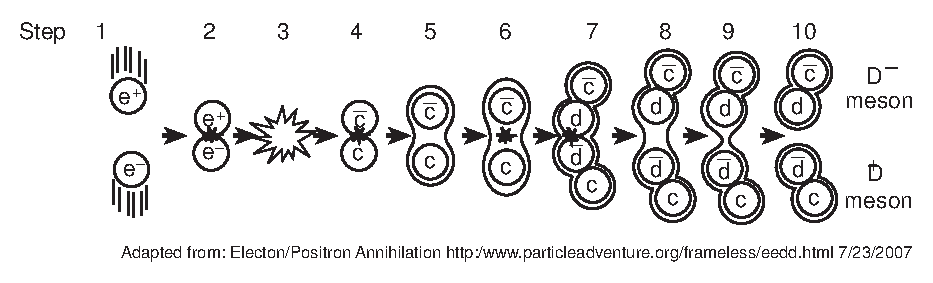
\includegraphics[width=0.95\columnwidth,keepaspectratio]{Jan2008-Q35}
    \end{center}
    Which statement best describes the changes that occur in this sequence of events?
    \begin{choices}
      \correctchoice{Energy is converted into matter and then matter is converted into energy.}
        \wrongchoice{Matter is converted into energy and then energy is converted into matter.}
        \wrongchoice{Isolated quarks are being formed from baryons.}
        \wrongchoice{Hadrons are being converted into leptons.}
    \end{choices}
\end{question}
}

\element{nysed}{
\begin{question}{Jan2008-Q45}
    A particle unaffected by an electric field could have a quark composition of:
    \begin{multicols}{2}
    \begin{choices}
      \correctchoice{$css$}
        \wrongchoice{$bbb$}
        \wrongchoice{$udc$}
        \wrongchoice{$uud$}
    \end{choices}
    \end{multicols}
\end{question}
}


%% Section June2007
%%--------------------
\element{nysed}{
\begin{question}{June2007-Q35}
    The energy produced by the complete conversion of \SI{2.0e-5}{\kilo\gram} of mass into energy is:
    \begin{multicols}{2}
    \begin{choices}
      \correctchoice{\SI{1.8}{\tera\joule}}
        \wrongchoice{\SI{6.0}{\giga\joule}}
        \wrongchoice{\SI{1.8}{\mega\joule}}
        \wrongchoice{\SI{6.0}{\kilo\joule}}
    \end{choices}
    \end{multicols}
\end{question}
}

\element{nysed}{
\begin{question}{June2007-Q45}
    Baryons may have charges of:
    \begin{multicols}{2}
    \begin{choices}
        \wrongchoice{$+1e$ and $+\frac{4}{3}e$}
        \wrongchoice{$+2e$ and $+3e$}
      \correctchoice{$-1e$ and $+1e$}
        \wrongchoice{$-2e$ and $-\frac{2}{3}e$}
    \end{choices}
    \end{multicols}
\end{question}
}


%% Section Jan2007
%%--------------------
\element{nysed}{
\begin{question}{Jan2007-Q16}
    Which statement best describes a proton that is being accelerated?
    \begin{choices}
      \correctchoice{It produces electromagnetic radiation.}
        \wrongchoice{The magnitude of its charge increases.}
        \wrongchoice{It absorbs a neutron to become an electron.}
        \wrongchoice{It is attracted to other protons.}
    \end{choices}
\end{question}
}

\element{nysed}{
\begin{question}{Jan2007-Q30}
    A photon having an energy of \SI{9.40}{\eV} strikes a hydrogen atom in the ground state.
    Why is the photon not absorbed by the hydrogen atom?
    \begin{choices}
        \wrongchoice{The atom's orbital electron is moving too fast.}
        \wrongchoice{The photon striking the atom is moving too fast.}
      \correctchoice{The photon's energy is too small.}
        \wrongchoice{The photon is being repelled by electrostatic force}
    \end{choices}
\end{question}
}

\element{nysed}{
\begin{question}{Jan2007-Q34}
    The charge of an antistrange quark is approximately:
    \begin{multicols}{2}
    \begin{choices}
      \correctchoice{\SI[retain-explicit-plus]{+5.33e-20}{\coulomb}}
        \wrongchoice{\SI[retain-explicit-plus]{-5.33e-20}{\coulomb}}
        \wrongchoice{\SI[retain-explicit-plus]{+5.33e20}{\coulomb}}
        \wrongchoice{\SI[retain-explicit-plus]{-5.33e20}{\coulomb}}
    \end{choices}
    \end{multicols}
\end{question}
}

\element{nysed}{
\begin{question}{Jan2007-Q35}
    What fundamental force holds quarks together to form particles such as protons and neutrons?
    \begin{choices}
        \wrongchoice{electromagnetic force}
        \wrongchoice{gravitational force}
      \correctchoice{strong force}
        \wrongchoice{weak force}
    \end{choices}
\end{question}
}

\element{nysed}{
\begin{question}{Jan2007-Q51}
    What is the total number of quarks in a helium nucleus consisting of 2 protons and 2 neutrons?
    \begin{multicols}{4}
    \begin{choices}
        \wrongchoice{16}
      \correctchoice{12}
        \wrongchoice{8}
        \wrongchoice{4}
    \end{choices}
    \end{multicols}
\end{question}
}


%% Section June2006
%%--------------------
\element{nysed}{
\begin{question}{June2006-Q34}
    A top quark has an approximate charge of:
    \begin{multicols}{2}
    \begin{choices}
        \wrongchoice{\SI{-1.07e-19}{\coulomb}}
        \wrongchoice{\SI{-2.40e-19}{\coulomb}}
      \correctchoice{\SI{+1.07e-19}{\coulomb}}
        \wrongchoice{\SI{+2.40e-19}{\coulomb}}
    \end{choices}
    \end{multicols}
\end{question}
}

\element{nysed}{
\begin{question}{June2006-Q35}
    A tritium nucleus is formed by combining two neutrons and a proton.
    The mass of this nucleus is \num{9.106e-3} universal mass unit less than the combined mass of the particles from which it is formed.
    Approximately how much energy is released when this nucleus is formed?
    \begin{multicols}{2}
    \begin{choices}
        \wrongchoice{\SI{8.48e-2}{\mega\eV}}
        \wrongchoice{\SI{2.73}{\mega\eV}}
      \correctchoice{\SI{8.48}{\mega\eV}}
        \wrongchoice{\SI{273}{\mega\eV}}
    \end{choices}
    \end{multicols}
\end{question}
}

\element{nysed}{
\begin{question}{June2006-Q50}
    Which type of photon is emitted when an electron in a hydrogen atom drops from the $n=2$ to the $n=1$ energy level?
    \begin{multicols}{2}
    \begin{choices}
      \correctchoice{ultraviolet}
        \wrongchoice{infrared}
        \wrongchoice{visible light}
        \wrongchoice{radio wave}
    \end{choices}
    \end{multicols}
\end{question}
}

\element{nysed}{
\begin{question}{June2006-Q51}
    A lithium atom consists of 3 protons,
        4 neutrons, and 3 electrons.
    This atom contains a total of:
    \begin{choices}
        \wrongchoice{9 quarks and 7 leptons}
        \wrongchoice{12 quarks and 6 leptons}
        \wrongchoice{14 quarks and 3 leptons}
      \correctchoice{21 quarks and 3 leptons}
    \end{choices}
\end{question}
}


%% Section Jan2006
%%--------------------
\element{nysed}{
\begin{question}{Jan2006-Q35}
    Which phenomenon best supports the theory that matter has a wave nature?
    \begin{choices}
        \wrongchoice{electron momentum}
      \correctchoice{electron diffraction}
        \wrongchoice{photon momentum}
        \wrongchoice{photon diffraction}
    \end{choices}
\end{question}
}

\element{nysed}{
\begin{question}{Jan2006-Q42}
    According to the Standard Model of Particle Physics,
        a meson is composed of:
    \begin{choices}
        \wrongchoice{a quark and a muon neutrino}
      \correctchoice{a quark and an antiquark}
        \wrongchoice{three quarks}
        \wrongchoice{a lepton and an antilepton}
    \end{choices}
\end{question}
}

\element{nysed}{
\begin{question}{Jan2006-Q47}
    The diagram below represents the bright-line spectra of four elements,
        $A$, $B$, $C$, and $D$, and the spectrum of an unknown gaseous sample.
    \begin{center}
        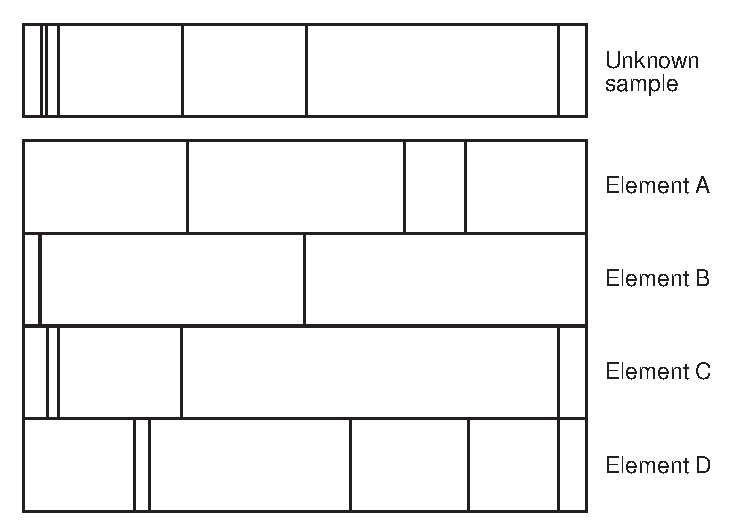
\includegraphics[width=0.95\columnwidth,keepaspectratio]{Jan2006-Q47}
    \end{center}
    Based on comparisons of these spectra,
        which two elements are found in the unknown sample?
    \begin{multicols}{2}
    \begin{choices}
        \wrongchoice{$A$ and $B$}
        \wrongchoice{$B$ and $C$}
        \wrongchoice{$A$ and $D$}
        \wrongchoice{$C$ and $D$}
    \end{choices}
    \end{multicols}
\end{question}
}


%% Section June2005
%%--------------------
\element{nysed}{
\begin{question}{June2005-Q32}
    Light of wavelength \SI{5.0e-7}{\meter} consists of photons having an energy of:
    \begin{multicols}{2}
    \begin{choices}
        \wrongchoice{\SI{1.1e-48}{\joule}}
        \wrongchoice{\SI{1.3e-27}{\joule}}
      \correctchoice{\SI{4.0e-19}{\joule}}
        \wrongchoice{\SI{1.7e-5}{\joule}}
    \end{choices}
    \end{multicols}
\end{question}
}

\element{nysed}{
\begin{question}{June2005-Q33}
    Wave-particle duality is most apparent in analyzing the motion of:
    \begin{multicols}{2}
    \begin{choices}
        \wrongchoice{a baseball}
        \wrongchoice{a galaxy}
        \wrongchoice{a space shuttle}
      \correctchoice{an electron}
    \end{choices}
    \end{multicols}
\end{question}
}

\element{nysed}{
\begin{question}{June2005-Q34}
    The tau neutrino, the muon neutrino,
        and the electron neutrino are all:
    \begin{multicols}{2}
    \begin{choices}
      \correctchoice{leptons}
        \wrongchoice{baryons}
        \wrongchoice{hadrons}
        \wrongchoice{mesons}
    \end{choices}
    \end{multicols}
\end{question}
}

\element{nysed}{
\begin{question}{June2005-Q35}
    Which statement is true of the strong nuclear force?
    \begin{choices}
        \wrongchoice{It acts over very great distances.}
        \wrongchoice{It holds protons and neutrons together.}
        \wrongchoice{It is much weaker than gravitational forces.}
        \wrongchoice{It repels neutral charges}
    \end{choices}
\end{question}
}

\element{nysed}{
\begin{question}{June2005-Q43}
    A hydrogen atom with an electron initially in the $n=2$ level is excited further until the electron is in the $n=4$ level.
    This energy level change occurs because the atom has:
    \begin{choices}
        \wrongchoice{absorbed a \SI{0.85}{\eV} photon}
      \correctchoice{absorbed a \SI{2.55}{\eV} photon}
        \wrongchoice{emitted a \SI{0.85}{\eV} photon}
        \wrongchoice{emitted a \SI{2.55}{\eV} photon}
    \end{choices}
\end{question}
}


%% Section Jan2005
%%--------------------
\element{nysed}{
\begin{question}{Jan2005-Q34}
    A meson may not have a charge of:
    \begin{multicols}{4}
    \begin{choices}
        \wrongchoice{$+1e$}
      \correctchoice{$+2e$}
        \wrongchoice{$0e$}
        \wrongchoice{$-1e$}
    \end{choices}
    \end{multicols}
\end{question}
}

\element{nysed}{
\begin{question}{Jan2005-Q43}
    According to the Standard Model,
        a proton is constructed of two up quarks and one down quark ($uud$) and a neutron is constructed of one up quark and two down quarks ($udd$).
    During beta decay,
        a neutron decays into a proton,
        an electron, and an electron antineutrino.
    During this process there is a conversion of a:
    \begin{choices}
      \correctchoice{$u$ quark to a $d$ quark}
        \wrongchoice{$d$ quark to a meson}
        \wrongchoice{baryon to another baryon}
        \wrongchoice{lepton to another lepton}
    \end{choices}
\end{question}
}

\element{nysed}{
\begin{question}{Jan2005-Q44}
    The bright-line emission spectrum of an element can best be explained by:
    \begin{choices}
        \wrongchoice{electrons transitioning between discrete energy levels in the atoms of that element.}
        \wrongchoice{protons acting as both particles and waves.}
        \wrongchoice{electrons being located in the nucleus.}
        \wrongchoice{protons being dispersed uniformly throughout the atoms of that element.}
    \end{choices}
\end{question}
}

\element{nysed}{
\begin{question}{Jan2005-Q45}
    How much energy is required to move an electron in a mercury atom from the ground state to energy level $h$?
    \begin{multicols}{2}
    \begin{choices}
        \wrongchoice{\SI{1.57}{\eV}}
      \correctchoice{\SI{8.81}{\eV}}
        \wrongchoice{\SI{10.38}{\eV}}
        \wrongchoice{\SI{11.95}{\eV}}
    \end{choices}
    \end{multicols}
\end{question}
}


%% Section June2004
%%--------------------
\element{nysed}{
\begin{question}{June2004-Q41}
    Which combination of quarks could produce a neutral baryon?
    \begin{multicols}{2}
    \begin{choices}
        \wrongchoice{$cdt$}
      \correctchoice{$cdb$}
        \wrongchoice{$cts$}
        \wrongchoice{$cdu$}
    \end{choices}
    \end{multicols}
\end{question}
}


%% Section Jan2004
%%--------------------
\element{nysed}{
\begin{question}{Jan2004-Q33}
    The charge-to-mass ratio of an electron is:
    \begin{multicols}{2}
    \begin{choices}
        \wrongchoice{\SI{5.69e-12}{\coulomb\per\kilo\gram}}
        \wrongchoice{\SI{1.76e-11}{\coulomb\per\kilo\gram}}
      \correctchoice{\SI{1.76e11}{\coulomb\per\kilo\gram}}
        \wrongchoice{\SI{5.69e12}{\coulomb\per\kilo\gram}}
    \end{choices}
    \end{multicols}
\end{question}
}

\element{nysed}{
\begin{question}{Jan2004-Q34}
    The force that holds protons and neutrons together is known as the:
    \begin{choices}
        \wrongchoice{gravitational force}
      \correctchoice{strong force}
        \wrongchoice{magnetic force}
        \wrongchoice{electrostatic force}
    \end{choices}
\end{question}
}

\element{nysed}{
\begin{question}{Jan2004-Q35}
    The energy equivalent of \SI{5.0e-3}{\kilo\gram} is:
    \begin{multicols}{2}
    \begin{choices}
        \wrongchoice{\SI{8.0e5}{\joule}}
        \wrongchoice{\SI{1.5e6}{\joule}}
      \correctchoice{\SI{4.5e14}{\joule}}
        \wrongchoice{\SI{3.0e19}{\joule}}
    \end{choices}
    \end{multicols}
\end{question}
}

\element{nysed}{
\begin{question}{Jan2004-Q47}
    An electron in a mercury atom drops from energy level $i$ to the ground state by emitting a single photon.
    This photon has an energy of:
    \begin{multicols}{2}
    \begin{choices}
        \wrongchoice{\SI{1.56}{\eV}}
      \correctchoice{\SI{8.82}{\eV}}
        \wrongchoice{\SI{10.38}{\eV}}
        \wrongchoice{\SI{11.94}{\eV}}
    \end{choices}
    \end{multicols}
\end{question}
}

\element{nysed}{
\begin{question}{Jan2004-Q48}
    Excited hydrogen atoms are all in the $n=3$ state.
    How many different photon energies could possibly be emitted as these atoms return to the ground state?
    \begin{multicols}{4}
    \begin{choices}
        \wrongchoice{\num{1}}
        \wrongchoice{\num{2}}
      \correctchoice{\num{3}}
        \wrongchoice{\num{4}}
    \end{choices}
    \end{multicols}
\end{question}
}


%% Section June2003
%%--------------------
\element{nysed}{
\begin{question}{June2003-Q31}
    White light is passed through a cloud of cool hydrogen gas and then examined with a spectroscope.
    The dark lines observed on a bright background are caused by:
    \begin{choices}
        \wrongchoice{the hydrogen emitting all frequencies in white light.}
      \correctchoice{the hydrogen absorbing certain frequencies of the white light.}
        \wrongchoice{diffraction of the white light.}
        \wrongchoice{constructive interference.}
    \end{choices}
\end{question}
}

\element{nysed}{
\begin{question}{June2003-Q33}
    Protons and neutrons are examples of:
    \begin{multicols}{2}
    \begin{choices}
        \wrongchoice{positrons}
        \wrongchoice{mesons}
      \correctchoice{baryons}
        \wrongchoice{quarks}
    \end{choices}
    \end{multicols}
\end{question}
}

\element{nysed}{
\begin{question}{June2003-Q34}
    The strong force is the force of:
    \begin{choices}
        \wrongchoice{repulsion between protons}
        \wrongchoice{attraction between protons and electrons}
        \wrongchoice{repulsion between nucleons}
        \wrongchoice{attraction between nucleons}
    \end{choices}
\end{question}
}

\element{nysed}{
\begin{question}{June2003-Q35}
    If a deuterium nucleus has a mass of \num{1.53e-3} universal mass units less than its components,
        this mass represents an energy of:
    \begin{multicols}{2}
    \begin{choices}
        \wrongchoice{\SI{1.38}{\mega\eV}}
        \wrongchoice{\SI{1.53}{\mega\eV}}
      \correctchoice{\SI{1.42}{\mega\eV}}
        \wrongchoice{\SI{3.16}{\mega\eV}}
    \end{choices}
    \end{multicols}
\end{question}
}

\element{nysed}{
\begin{question}{June2003-Q41}
    Which combination of quarks could produce a neutral baryon?
    \begin{multicols}{2}
    \begin{choices}
        \wrongchoice{$cdt$}
      \correctchoice{$cdb$}
        \wrongchoice{$cts$}
        \wrongchoice{$cdu$}
    \end{choices}
    \end{multicols}
\end{question}
}


%% Section Jan2003
%%--------------------


%% Section Aug2002
%%--------------------
\element{nysed}{
\begin{question}{Aug2002-Q23}
    After electrons in hydrogen atoms are excited to the $n=3$ energy state,
        how many different frequencies of radiation can be emitted as the electrons return to the ground state?
    \begin{multicols}{4}
    \begin{choices}
        \wrongchoice{\num{1}}
        \wrongchoice{\num{2}}
      \correctchoice{\num{3}}
        \wrongchoice{\num{4}}
    \end{choices}
    \end{multicols}
\end{question}
}

\element{nysed}{
\begin{question}{Aug2002-Q24}
    What type of nuclear force holds the protons and neutrons in an atom together?
    \begin{choices}
      \correctchoice{a strong force that acts over a short range}
        \wrongchoice{a strong force that acts over a long range}
        \wrongchoice{a weak force that acts over a short range}
        \wrongchoice{a weak force that acts over a long range}
    \end{choices}
\end{question}
}

\element{nysed}{
\begin{question}{Aug2002-Q44}
    Which combination of quarks would produce a neutral baryon?
    \begin{multicols}{2}
    \begin{choices}
        %% NOTE: Change formatting and check answer
        \wrongchoice{$uud$}
        \wrongchoice{$udd$}
        \wrongchoice{$\bar{u}\bar{u}d$}
        \wrongchoice{$\bar{u}dd$}
    \end{choices}
    \end{multicols}
\end{question}
}

%\element{nysed}{
%\begin{question}{Aug2002-Q47}
%    In the cartoon,
%    %% NOTE: graphic cannot be tikz
%        Einstein is contemplating the equation for the principle that:
%    \begin{choices}
%        \wrongchoice{the fundamental source of all energy is the conversion of mass into energy.}
%        \wrongchoice{energy is emitted or absorbed in discrete packets called photons.}
%        \wrongchoice{mass always travels at the speed of light in a vacuum.}
%        \wrongchoice{the energy of a photon is proportional to its frequency.}
%    \end{choices}
%\end{question}
%}


%% Section June2002
%%--------------------
\element{nysed}{
\begin{question}{June2002-Q40}
    What is the minimum energy needed to ionize a hydrogen atom in the $n=2$ energy state?
    \begin{multicols}{2}
    \begin{choices}
        \wrongchoice{\SI{13.6}{\eV}}
      \correctchoice{\SI{3.40}{\eV}}
        \wrongchoice{\SI{10.2}{\eV}}
        \wrongchoice{\SI{1.89}{\eV}}
    \end{choices}
    \end{multicols}
\end{question}
}


%% Section Jan2002
%%--------------------
\element{nysed}{
\begin{question}{Jan2002-Q51}
    An electron in a hydrogen atom drops from the $n=3$ energy level to the $n=2$ energy level.
    The energy of the emitted photon is:
    \begin{multicols}{2}
    \begin{choices}
        \wrongchoice{\SI{1.51}{\eV}}
      \correctchoice{\SI{1.89}{\eV}}
        \wrongchoice{\SI{3.40}{\eV}}
        \wrongchoice{\SI{4.91}{\eV}}
    \end{choices}
    \end{multicols}
\end{question}
}


%% Section June2001
%%--------------------
\element{nysed}{
\begin{question}{June2001-Q48}
    Alpha particles were directed at a thin metal foil.
    Some particles were deflected into hyperbolic paths due to:
    \begin{choices}
        \wrongchoice{gravitational attraction}
      \correctchoice{electrostatic repulsion}
        \wrongchoice{electrostatic attraction}
        \wrongchoice{magnetic repulsion}
    \end{choices}
\end{question}
}

\element{nysed}{
\begin{question}{June2001-Q49}
    The threshold frequency in a photoelectric experiment is most closely related to the:
    \begin{choices}
        \wrongchoice{brightness of the incident light}
        \wrongchoice{thickness of the photoemissive metal}
        \wrongchoice{area of the photoemissive metal}
      \correctchoice{work function of the photoemissive metal}
    \end{choices}
\end{question}
}

\element{nysed}{
\begin{question}{June2001-Q50}
    The momentum of a photon is inversely proportional to the photon's:
    \begin{multicols}{2}
    \begin{choices}
        \wrongchoice{frequency}
        \wrongchoice{weight}
        \wrongchoice{mass}
        \wrongchoice{wavelength}
    \end{choices}
    \end{multicols}
\end{question}
}

\element{nysed}{
\begin{question}{June2001-Q51}
    The electron in a hydrogen atom drops from energy level $n=2$ to energy level $n=1$ by emitting a photon having an energy of approximately:
    \begin{multicols}{2}
    \begin{choices}
      \correctchoice{\SI{5.4e-19}{\joule}}
        \wrongchoice{\SI{1.6e-18}{\joule}}
        \wrongchoice{\SI{2.2e-18}{\joule}}
        \wrongchoice{\SI{7.4e-18}{\joule}}
    \end{choices}
    \end{multicols}
\end{question}
}

\element{nysed}{
\begin{question}{June2001-Q52}
    In the currently accepted model of the atom,
        a fuzzy cloud around a hydrogen nucleus is used to represent the:
    \begin{choices}
        \wrongchoice{electron's actual path, which is not a circular orbit.}
        \wrongchoice{general region where the atom's proton is most probably located.}
        \wrongchoice{general region where the atom's electron is most probably located.}
        \wrongchoice{presence of water vapor in the atom.}
    \end{choices}
\end{question}
}

\element{nysed}{
\begin{question}{June2001-Q81}
    The diagram below shows a proton moving with velocity $v$ about to enter a uniform magnetic field directed into the page.
    As the proton moves into the magnetic field,
        the magnitude of the magnetic force on the proton is $F$.
    \begin{center}
    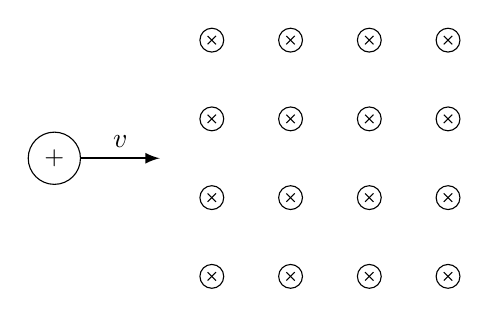
\begin{tikzpicture}
        %% B field into page
        \foreach \x in {0,1,2,3}
            \foreach \y in {0,1,2,3} {
                \draw (\x,\y) circle (1ex);
                \foreach \z in {45,135,225,315}
                    \draw (\x,\y) -- ++(\z:0.5ex);
            }
        %% proton with velocity
        \node[font=\small,anchor=center,circle,draw] (A) at (-2,1.5) {$+$};
        \draw[thick,-latex] (A.east) -- ++(0:1) node[pos=0.5,anchor=south] {$v$};
    \end{tikzpicture}
    \end{center}
    If the proton were replaced by an alpha particle under the same conditions,
        the magnitude of the magnetic force on the alpha particle would be:
    \begin{multicols}{4}
    \begin{choices}
        \wrongchoice{$F$}
      \correctchoice{$2 F$}
        \wrongchoice{$\dfrac{F}{2}$}
        \wrongchoice{$4 F$}
    \end{choices}
    \end{multicols}
\end{question}
}

\element{nysed}{
\begin{question}{June2001-Q82}
    The isotopes of an element can be separated using a:
    \begin{multicols}{2}
    \begin{choices}
        \wrongchoice{cathode ray tube}
        \wrongchoice{diffraction grating}
        \wrongchoice{Geiger counter}
      \correctchoice{mass spectrometer}
    \end{choices}
    \end{multicols}
\end{question}
}

\element{nysed}{
\begin{question}{June2001-Q85}
    What is the origin of the light emitted by a laser?
    \begin{choices}
        \wrongchoice{thermionic emission from an incandescent filament}
        \wrongchoice{emission of mechanical waves from vibrating matter}
        \wrongchoice{emission of photoelectrons from a photosensitive surface}
      \correctchoice{emission of photons from excited atoms}
    \end{choices}
\end{question}
}


%% Section Jan2001
%%--------------------
\element{nysed}{
\begin{question}{Jan2001-Q55}
    Photons with an energy of \SI{7.9}{\eV} strike a zinc plate,
        causing the emission of photoelectrons with a maximum kinetic energy of \SI{4.0}{\eV}.
    The work function of the zinc plate is:
    \begin{multicols}{2}
    \begin{choices}
        \wrongchoice{\SI{11.9}{\eV}}
        \wrongchoice{\SI{7.9}{\eV}}
      \correctchoice{\SI{3.9}{\eV}}
        \wrongchoice{\SI{4.0}{\eV}}
    \end{choices}
    \end{multicols}
\end{question}
}


%% Section June2000
%%--------------------
\element{nysed}{
\begin{question}{June2000-Q53}
    A beam of monochromatic light incident on a metal surface causes the emission of photoelectrons.
    The length of time that the surface is illuminated by this beam is varied,
        but the intensity of the beam is kept constant.
    Which graph best represents the relationship between the total number of photoelectrons emitted and the length of time of illumination?
    \begin{multicols}{2}
    \begin{choices}
        \AMCboxDimensions{down=-2.5em}
        \correctchoice{
            \begin{tikzpicture}
                \begin{axis}[
                    axis y line=left,
                    axis x line=bottom,
                    axis line style={->},
                    xlabel={photoelectrons},
                    xtick=\empty,
                    ylabel={time},
                    ytick=\empty,
                    xmin=0,xmax=11,
                    ymin=0,ymax=11,
                    width=\columnwidth,
                    very thin,
                ]
                \addplot[line width=1pt,domain=0:10]{x};
                \end{axis}
            \end{tikzpicture}
        }
        \wrongchoice{
            \begin{tikzpicture}
                \begin{axis}[
                    axis y line=left,
                    axis x line=bottom,
                    axis line style={->},
                    xlabel={photoelectrons},
                    xtick=\empty,
                    ylabel={time},
                    ytick=\empty,
                    xmin=0,xmax=11,
                    ymin=0,ymax=11,
                    width=\columnwidth,
                    very thin,
                ]
                \addplot[line width=1pt,domain=0:10]{8};
                \end{axis}
            \end{tikzpicture}
        }
        \wrongchoice{
            \begin{tikzpicture}
                \begin{axis}[
                    axis y line=left,
                    axis x line=bottom,
                    axis line style={->},
                    xlabel={photoelectrons},
                    xtick=\empty,
                    ylabel={time},
                    ytick=\empty,
                    xmin=0,xmax=11,
                    ymin=0,ymax=11,
                    width=\columnwidth,
                    very thin,
                ]
                \addplot[line width=1pt,domain=0:10]{10-x};
                \end{axis}
            \end{tikzpicture}
        }
        \wrongchoice{
            \begin{tikzpicture}
                \begin{axis}[
                    axis y line=left,
                    axis x line=bottom,
                    axis line style={->},
                    xlabel={photoelectrons},
                    xtick=\empty,
                    ylabel={time},
                    ytick=\empty,
                    xmin=0,xmax=11,
                    ymin=0,ymax=11,
                    width=\columnwidth,
                    very thin,
                ]
                \addplot[line width=1pt,domain=0:10]{10/x};
                \end{axis}
            \end{tikzpicture}
        }
    \end{choices}
    \end{multicols}
\end{question}
}

\element{nysed}{
\begin{question}{June2000-Q54}
    What is the minimum energy required to excite a mercury atom initially in the ground state?
    \begin{multicols}{2}
    \begin{choices}
      \correctchoice{\SI{4.64}{\eV}}
        \wrongchoice{\SI{10.20}{\eV}}
        \wrongchoice{\SI{5.74}{\eV}}
        \wrongchoice{\SI{10.38}{\eV}}
    \end{choices}
    \end{multicols}
\end{question}
}

\element{nysed}{
\begin{question}{June2000-Q55}
    The diagram below represents the hyperbolic path of an alpha particle as it passes very near the nucleus of a gold atom.
    \begin{center}
    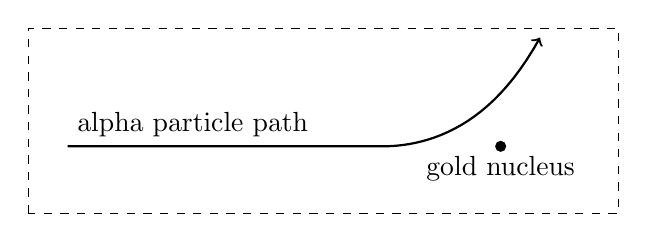
\begin{tikzpicture}
        \def\a{0.5}
        %% personal
        \draw[dashed] (-4.5,-1em) rectangle (3,2);
        \node[anchor=south west] at (-4,\a) {alpha particle path};
        \draw[thick,->] (-4,\a) -- (0,\a)  plot[domain=0:2] (\x,{\a*cosh(\x)});
        \fill (1.5,\a) circle (2pt) node[anchor=north] {gold nucleus};
    \end{tikzpicture}
    \end{center}
    The shape of the path is caused by the force between the:
    \begin{choices}
        \wrongchoice{positively charged alpha particle and the neutral nucleus.}
      \correctchoice{positively charged alpha particle and the positively charged nucleus.}
        \wrongchoice{negatively charged alpha particle and the neutral nucleus.}
        \wrongchoice{negatively charged alpha particle and the positively charged nucleus.}
    \end{choices}
\end{question}
}


%% Section June1999
%%--------------------


%% Section June1998
%%--------------------

%% NOTE: June1998-Q47: tikz?


%% Section June1997
%%--------------------
\element{nysed}{
\begin{question}{June1997-Q49}
    When \SI{8.0}{\eV} photons strike a photoemissive surface,
        the maximum kinetic energy of ejected photoelectrons is \SI{6.0}{\eV}.
    The work function of the photoemissive surface is:
    \begin{multicols}{2}
    \begin{choices}
        \wrongchoice{\SI{0.0}{\eV}}
      \correctchoice{\SI{2.0}{\eV}}
        \wrongchoice{\SI{7.0}{\eV}}
        \wrongchoice{\SI{14.0}{\eV}}
    \end{choices}
    \end{multicols}
\end{question}
}

\element{nysed}{
\begin{question}{June1997-Q50}
    If the momentum of a particle is \SI{1.8e-22}{\kilo\meter\per\second},
        its matter wavelength is approximately:
    \begin{multicols}{2}
    \begin{choices}
        \wrongchoice{\SI{1.2e-55}{\meter}}
        \wrongchoice{\SI{2.7e11}{\meter}}
      \correctchoice{\SI{3.7e-12}{\meter}}
        \wrongchoice{\SI{5.0e-7}{\meter}}
    \end{choices}
    \end{multicols}
\end{question}
}

\element{nysed}{
\begin{question}{June1997-Q51}
    The threshold frequency of a photoemissive surface is \SI{7.1e14}{\hertz}.
    Which electromagnetic radiation, incident upon the surface,
        will produce the greatest amount of current?
    \begin{choices}
        \wrongchoice{low intensity infrared radiation}
        \wrongchoice{high intensity infrared radiation}
        \wrongchoice{low intensity ultraviolet radiation}
      \correctchoice{high intensity ultraviolet radiation}
    \end{choices}
\end{question}
}

\element{nysed}{
\begin{question}{June1997-Q52}
    Which diagram shows a possible path of an alpha particle as it passes very near the nucleus of a gold atom?
    \begin{choices}
        \AMCboxDimensions{down=-0.8cm}
        \correctchoice{
            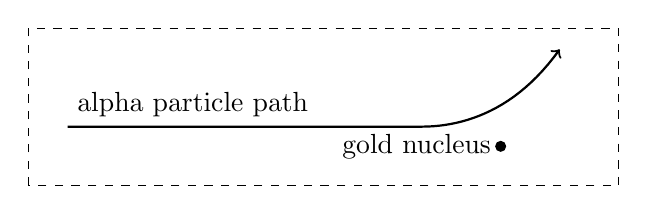
\begin{tikzpicture}
                \draw[dashed] (-4.5,-0.25) rectangle (3,1.75);
                \node[anchor=south west] at (-4,0.5) {alpha particle path};
                \draw[thick,->] (-4,0.5) -- (0.5,0.5)  plot[domain=0:1.75] ({\x +0.5},{0.5*cosh(\x)});
                \fill (1.5,0.25) circle (2pt) node[anchor=east] {gold nucleus};
            \end{tikzpicture}
        }
        \wrongchoice{
            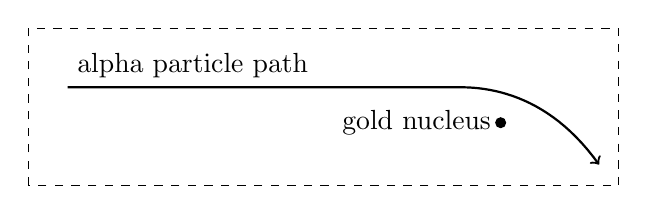
\begin{tikzpicture}
                \draw[dashed] (-4.5,-0.25) rectangle (3,1.75);
                \node[anchor=south west] at (-4,1) {alpha particle path};
                \draw[thick,->] (-4,1) -- (1,1)  plot[domain=0:1.75] ({\x + 1.0},{1.5-0.5*cosh(\x)});
                \fill (1.5,0.55) circle (2pt) node[anchor=east] {gold nucleus};
            \end{tikzpicture}
        }
        \wrongchoice{
            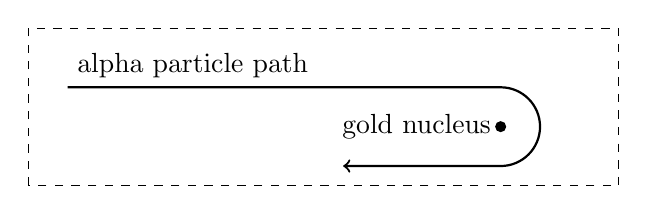
\begin{tikzpicture}
                \draw[dashed] (-4.5,-0.5) rectangle (3,1.5);
                \node[anchor=south west] at (-4,0.75) {alpha particle path};
                \draw[thick,->] (-4,0.75) -- (1.5,0.75) arc(90:-90:0.5) -- ++(180:2);
                \fill (1.5,0.25) circle (2pt) node[anchor=east] {gold nucleus};
            \end{tikzpicture}
        }
        \wrongchoice{
            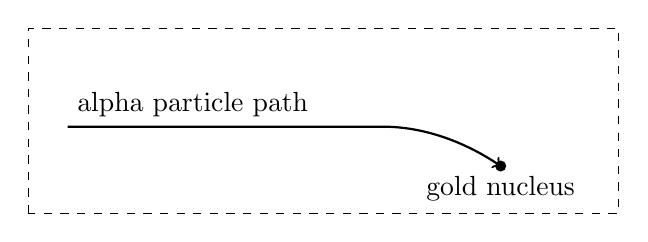
\begin{tikzpicture}
                \draw[dashed] (-4.5,-1em) rectangle (3,2);
                \node[anchor=south west] at (-4,0.75) {alpha particle path};
                \draw[thick,->] (-4,0.75) -- (0,0.75) parabola (1.5,0.25);
                \fill (1.5,0.25) circle (2pt) node[anchor=north] {gold nucleus};
            \end{tikzpicture}
        }
    \end{choices}
\end{question}
}

\element{nysed}{
\begin{question}{June1997-Q53}
    A hydrogen atom could have an electron energy-level transition from $n=2$ to $n=3$ by absorbing a photon having an energy of:
    \begin{multicols}{2}
    \begin{choices}
        \wrongchoice{\SI{1.51}{\eV}}
      \correctchoice{\SI{1.89}{\eV}}
        \wrongchoice{\SI{4.91}{\eV}}
        \wrongchoice{\SI{10.20}{\eV}}
    \end{choices}
    \end{multicols}
\end{question}
}


%% Section June1996
%%--------------------
\element{nysed}{
\begin{question}{June1996-Q48}
    Which phenomenon is most easily explained by the particle theory of light?
    \begin{choices}
        \wrongchoice{photoelectric effect}
        \wrongchoice{constructive interference}
        \wrongchoice{polarization}
        \wrongchoice{diffraction}
    \end{choices}
\end{question}
}

\element{nysed}{
\begin{question}{June1996-Q49}
    The work function for a copper surface is \SI{7.3e-12}{\joule}.
    If photons with an energy of \SI{9.9e-19}{\joule} are incident on the copper surface,
        the maximum kinetic energy of the ejected photoelectrons is:
    \begin{multicols}{2}
    \begin{choices}
      \correctchoice{\SI{2.6e-19}{\joule}}
        \wrongchoice{\SI{7.3e-19}{\joule}}
        \wrongchoice{\SI{9.9e-19}{\joule}}
        \wrongchoice{\SI{1.7e-19}{\joule}}
    \end{choices}
    \end{multicols}
\end{question}
}

\element{nysed}{
\begin{question}{June1996-Q51}
    What is the minimum energy required to ionize a hydrogen atom in the $n=3$ state?
    \begin{multicols}{2}
    \begin{choices}
        \wrongchoice{\SI{13.60}{\eV}}
        \wrongchoice{\SI{12.09}{\eV}}
        \wrongchoice{\SI{5.52}{\eV}}
      \correctchoice{\SI{1.51}{\eV}}
    \end{choices}
    \end{multicols}
\end{question}
}

\element{nysed}{
\begin{question}{June1996-Q52}
    When a source of dim orange light shines on a photosensitive metal,
        no photoelectrons are ejected from it surface.
    What could be done to increase the likelihood of producing photoelectrons?
    \begin{choices}
        \wrongchoice{Replace the orange light source with a red light source.}
      \correctchoice{Replace the orange light source with a higher frequency light source.}
        \wrongchoice{Increase the brightness of the orange light source.}
        \wrongchoice{Increase the angle at which the photons of orange light strike the metal.}
    \end{choices}
\end{question}
}

\element{nysed}{
\begin{question}{June1996-Q53}
    In Rutherford's model of the atom, the positive charge:
    \begin{choices}
        \wrongchoice{is distributed throughout the atom's volume.}
        \wrongchoice{revolves about the nucleus in specific orbits.}
      \correctchoice{is concentrated at the center of the atom.}
        \wrongchoice{occupies most of the space in the atom.}
    \end{choices}
\end{question}
}


%% Section June1990
%%--------------------
\element{nysed}{
\begin{question}{June1990-Q54}
    Which graph best represents the relationship between the photocurrent in a photoelectric cell and the intensity of the incident light?
    \begin{multicols}{2}
    \begin{choices}
        \AMCboxDimensions{down=-2.5em}
        %% ANS is 1
        \correctchoice{
            \begin{tikzpicture}
                \begin{axis}[
                    axis y line=left,
                    axis x line=bottom,
                    axis line style={->},
                    xlabel={intensity},
                    xtick=\empty,
                    ylabel={photocurrent},
                    ytick=\empty,
                    xmin=0,xmax=11,
                    ymin=0,ymax=11,
                    width=\columnwidth,
                    very thin,
                ]
                \addplot[line width=1pt,domain=0:10]{x};
                \end{axis}
            \end{tikzpicture}
        }
        \wrongchoice{
            \begin{tikzpicture}
                \begin{axis}[
                    axis y line=left,
                    axis x line=bottom,
                    axis line style={->},
                    xlabel={intensity},
                    xtick=\empty,
                    ylabel={photocurrent},
                    ytick=\empty,
                    xmin=0,xmax=11,
                    ymin=0,ymax=11,
                    width=\columnwidth,
                    very thin,
                ]
                \addplot[line width=1pt,domain=0:10]{10-x};
                \end{axis}
            \end{tikzpicture}
        }
        \wrongchoice{
            \begin{tikzpicture}
                \begin{axis}[
                    axis y line=left,
                    axis x line=bottom,
                    axis line style={->},
                    xlabel={intensity},
                    xtick=\empty,
                    ylabel={photocurrent},
                    ytick=\empty,
                    xmin=0,xmax=11,
                    ymin=0,ymax=11,
                    width=\columnwidth,
                    very thin,
                ]
                \addplot[line width=1pt,domain=0:10]{6};
                \end{axis}
            \end{tikzpicture}
        }
        \wrongchoice{
            \begin{tikzpicture}
                \begin{axis}[
                    axis y line=left,
                    axis x line=bottom,
                    axis line style={->},
                    xlabel={intensity},
                    xtick=\empty,
                    ylabel={photocurrent},
                    ytick=\empty,
                    xmin=0,xmax=11,
                    ymin=0,ymax=11,
                    width=\columnwidth,
                    very thin,
                ]
                \addplot[line width=1pt,domain=0:10]{10/x};
                \end{axis}
            \end{tikzpicture}
        }
    \end{choices}
    \end{multicols}
\end{question}
}

\element{nysed}{
\begin{question}{June1990-Q55}
    The threshold frequency for a photoemissive surface is \SI{4.0e14}{\hertz}.
    What is the work function of this surface?
    \begin{multicols}{2}
    \begin{choices}
        \wrongchoice{\SI{1.2e-19}{\joule}}
      \correctchoice{\SI{2.6e-19}{\joule}}
        \wrongchoice{\SI{6.0e14}{\joule}}
        \wrongchoice{\SI{6.1e47}{\joule}}
    \end{choices}
    \end{multicols}
\end{question}
}

\element{nysed}{
\begin{question}{June1990-Q56}
    The concept that electrons exhibit wave properties can best be demonstrated by the:
    \begin{choices}
        \wrongchoice{emission of photoelectrons}
        \wrongchoice{scattering of alpha particles by electrons}
        \wrongchoice{collisions between photons and electrons}
      \correctchoice{production of electron interference patterns}
    \end{choices}
\end{question}
}

\element{nysed}{
\begin{question}{June1990-Q57}
    According to the Rutherford model of the atom,
        an atomic nucleus contains:
    \begin{choices}
        \wrongchoice{all of the atom's electric charge, but none of the atom's mass}
        \wrongchoice{all of the atom's mass, but none of the atom's electric charge}
        \wrongchoice{most of the atom's mass and all of the atom's negative charge}
      \correctchoice{most of the atom's mass and all of the atom's positive charge}
    \end{choices}
\end{question}
}


%% Section June1989
%%--------------------
\element{nysed}{
\begin{question}{June1989-Q19}
    A \SI{2.0}{\kilo\gram} rifle initially at rest fires a \SI{0.002}{\kilo\gram} bullet.
    As the bullet leaves the rifle with a velocity of \SI{500}{\meter\per\second},
        what is the momentum of the rifle-bullet system?
    \begin{multicols}{2}
    \begin{choices}
        \wrongchoice{\SI{2.5}{\kilo\gram\meter\per\second}}
        \wrongchoice{\SI{2.0}{\kilo\gram\meter\per\second}}
        \wrongchoice{\SI{0.5}{\kilo\gram\meter\per\second}}
        %\correctchoice{zero}
      \correctchoice{\SI{0}{\kilo\gram\meter\per\second}}
    \end{choices}
    \end{multicols}
\end{question}
}


\endinput


